\documentclass[hidelinks, 11 pt]{article}

\usepackage[a4paper, top=12.7mm, bottom=25.4mm, left=19.1mm, right=19.1mm, footskip=8mm]{geometry}
\usepackage[skip=7pt]{parskip}
\usepackage[list=true, listformat=simple]{subcaption}
\usepackage{graphicx}
\usepackage{float}
\usepackage{amsthm}
\usepackage{amsmath}
\usepackage{fancyvrb}
\usepackage{hyperref}
\usepackage{pgfplots}
\usepackage{listings}
\usepackage{lstautogobble}
\usepackage[export]{adjustbox}

\pgfplotsset{compat=1.18}
\newsavebox{\imagebox}

\fvset{tabsize=4} % Set tabsize in Verbatim environments
\newcommand{\myhline}{\hline\noalign{\vskip 2pt}} % Space after hline
\renewcommand{\arraystretch}{1.2} % Increase spacing between rows of tables

% Penalties
\interfootnotelinepenalty=10000 % Force footnotes not to split over pages
\linepenalty=500 % Avoid runts
\hyphenpenalty=1000 % Avoid splitting words across lines by hyphenating
\clubpenalty=10000 % Avoid widows

% Format listings environments
\lstset{
	basicstyle=\ttfamily,
	columns=fullflexible,
	keepspaces=true,
	breaklines=true,
	autogobble=true,
	tabsize=4
}

% Format links
\hypersetup{
	colorlinks=false,
	linkbordercolor=black
}

\begin{document}

\begin{center}
	\huge The Case for \LaTeX\  \\
	\vspace{5mm}
	\large Henry Ginn  \\
	\vspace{3 mm}
	\large \today
\end{center}

\tableofcontents

\newpage

\section{Introduction}
\label{sec:Introduction}

This document gives a brief overview of what \LaTeX\ (pronounced ``Lay-tek") is and highlights some of the advantages it has over Microsoft Word. In a sentence, \LaTeX\ is a well-established piece of typesetting software for producing technical documents where the input is given in plain text which is then compiled into a PDF. I believe that using \LaTeX\ will improve upon several weaknesses in our document production and document control processes and is in line with our digital philosophy of using technology to improve our workflow. It is understandable why one may be wary of any potential barriers to those less comfortable with technology, but the payoff is more than worth it. The main advantages are as follows:

\begin{itemize}
	\item No need to worry about formatting - template is followed automatically.
	\item Equations, cross-references, and citations are far easier than in Word.
	\item Compatible with text-based version control systems such as Git.
	\item The \LaTeX\ compiler knows how to typeset better than you do so documents look professional.
	\item Less buggy than Word.
	\item Vector image compatible and are given by reference.
\end{itemize}

Below I have included the code used to create this section as an example of what \LaTeX\ may look like to a typical user\footnote{Note that this is done by reference to a file so it will update whenever this introduction is changed. This ``single source of truth" functionality is common in \LaTeX.}. Pressing the compile button converts this into a PDF.
\lstinputlisting{Introduction.tex}
\newpage

\section{Formatting}
\label{sec:Formatting}

We begin by outlining the problems with formatting in Word, even by a trained practitioner who knows how to use Word properly.

A document with poor or inconsistent formatting makes WSP look unprofessional, but fixing formatting is not something we should need to waste our time or client's money on. \LaTeX\ ensures formatting is consistent by defining it in one place only and applying globally it across the document. Once a template is defined, the formatting is abstracted away from the writer so they can focus soley on the content.

Some may argue that Word can do this through the styles feature, but it is easy to break the template in Word. For example, many times I have had section numbering disappear even though the numbering is part of the section header style and where reapplying the style did not fix it. In my experience, styles do not work reliably in tables either and properties such as spacing after paragraph need to be manually corrected around tables and figures. Once the template is defined the user should not need to put any extra work into ensuring that it is followed - the software should handle this for us.

Often I find Word does weird things that no one understands and there is no good fix. For example, I have had tables where the boldness of text would not save and the \href{https://learn.microsoft.com/en-us/answers/questions/5092571/tables-in-ms-word-are-changing-when-saved-and-re-o}{\underline{typical solution}} to a problem like this is to recreate the whole table from scratch or copy and paste everything into a new document. I have seen colleagues input tables as images rather than deal with Word's formatting, a veritable crime against typesetting that looks extremely unprofessional (this also means you cannot search or easily copy text in the table).

In \LaTeX, all formatting rules for elements such as section and subsection styles, spacing, font sizes, headers and footers, et cetera are defined at the start of the document. The template applies globally\footnote{It is possible to deviate from the template locally if you really want to but typically this is awkward to do. This is because you are trying to defy the compiler which almost always means you are attempting to commit crimes against typesetting and should not be doing whatever you are trying to do.} which makes documents look consistent and therefore only the type of formatting needs to be given. As examples, to tell the compiler you are creating new section or subsection, one would write \lstinline_\section{Example Section Name}_ or \lstinline_\subsection{Example Subsection Name}_ respectively and to tell it to format as a bullet point list, the following code is used.

\begin{lstlisting}
\begin{itemize}
	\item Example of the first item
	\item Example of the second item
\end{itemize}
\end{lstlisting}

\LaTeX\ also allows for more advanced features than Word and gives a lot more control. As simple examples, it is possible to adjust how much weight it should give towards avoiding widows, or exactly how much space you want between two elements. For a more complicated example, WSP recently changed the template used for CVs and each employee had to move to the new template. With \LaTeX\ this could have been done with a simple script to swap out the file that defined the formatting and then recompiled all CVs with the new template. A competant system administrator could have done this in a few minutes, yet instead this task needed to be done individually by thousands of people.\newpage
\section{Technical Writing}
\label{sec:TechnicalWriting}

One of the main powers of \LaTeX\ is the ability to format mathematics. In equation~\eqref{eqn:ClosureOfSO2} below is a simple example showing closure of the $SO(2)$ group, something that would be extremely painful to typeset in Word but is trivial to do in \LaTeX.

\begin{subequations}
\begin{align}
	R(\theta)R(\phi) &= 
	\left( \begin{array}{cc}
		\cos\theta & -\sin\theta \\
		\sin\theta & \cos\theta
	\end{array} \right)
	\left( \begin{array}{cc}
		\cos\phi & -\sin\phi \\
		\sin\phi & \cos\phi
	\end{array} \right)\label{eqn:ClosureOfSO2a}  \\
	&= \left( \begin{array}{cc}
		\cos\theta\cos\phi - \sin\theta\sin\phi & -\cos\theta\sin\phi -\sin\theta\cos\phi \\
		\sin\theta\cos\phi + \cos\theta\sin\phi & -\sin\theta\sin\phi + \cos\theta\cos\phi
	\end{array} \right)\label{eqn:ClosureOfSO2b}  \\
	&= \left( \begin{array}{cc}
		\cos(\theta + \phi) & -\sin(\theta + \phi) \\
		\sin(\theta + \phi) & \cos(\theta + \phi)
	\end{array} \right)\label{eqn:ClosureOfSO2c}  \\
	&= R(\theta + \phi)\label{eqn:ClosureOfSO2d}
\end{align}
\label{eqn:ClosureOfSO2}
\end{subequations}

We note the following that are impossible, awkward, or very manual to do in Word:

\begin{itemize}
	\item The equations are numbered automatically and we do not need to position them ourselves.
	\item The equations are aligned on the equals sign - I did not need to add spaces to do this.
	\item The whole equation or individual parts such as equation~\eqref{eqn:ClosureOfSO2b} can be cross-referenced easily.
	\item Much more complicated configurations can be created, such as equations in two columns.
\end{itemize}

Images are inserted by giving a path to the image. This means that the document also updates when images are updated when it is recompiled. Copying by reference means there is one version of the truth which is one of the reasons why copying by value in situations like this is poor practice. I have needed to spend a lot of time reinserting images into documents because it appears Word can only copy by value.

Word and other Microsoft Office Suite products are very poor at handling vector graphics. As an engineering consultancy, we feature many images which could be vector graphics yet are forced to be rasterised, lowering their quality. The only option I have found that Word is happy with are Enhanced Metafiles (EMF), a format of Microsoft's creation with many problems\footnote{EMF files do not support transparency. They also do not support antialiasing so all text looks odd as well.}. On the other hand, \LaTeX\ handles both bitmaps and vector graphics easily.

Word's strange behaviour with images and exporting wastes time. Word will compress images for you by default when pasting an image into the document, and even stranger, the level of compression depends on the zoom level of the editor. I have also seen documents where all the figures are unreadable because Word decided to compress them between revisions. There are many ways to export to PDF in Word, all of which behave differently and all of which compress images no matter what settings are used. \LaTeX\ will produce a PDF with the exact images it was given.

Going further than this, plots and figures can even be created inside \LaTeX\ itself, although this is typically for more advanced users. This means the font in plot titles and axis labels can be consistent with the rest of the document and even the entire project. I have not found any other way of achieving this conveniently for figures that scale to the given size automatically. Figure~\ref{fig:ExamplePlots} demonstrates the difference in quality. Even though figure~\ref{fig:ExampleRasterImage} has been well-made in Python, the lower resolution, inconsistent style, and nasty typesetting of $\pi$ symbols make it look noticibly worse than figure~\ref{fig:ExampleVectorImage}. Figure~\ref{fig:ExampleVectorImage} has infinite resolution and the added benefit of highlightable and searchable text\footnote{It is not necessary to make the figure in \LaTeX\ for this functionality, any vector image would have this.}.

\begin{figure}[H]
	\centering
	\begin{subfigure}{0.49\textwidth}
		\centering
		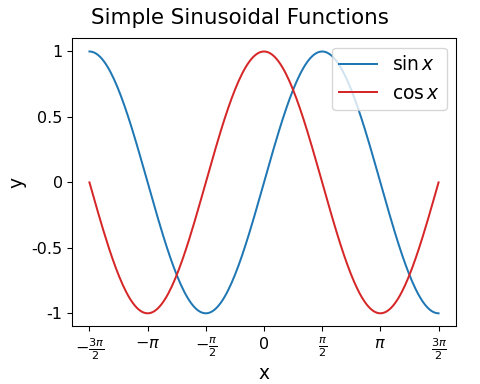
\includegraphics[width=\textwidth]{Figures/example_figure_matplotlib_096.png}
		\caption{96 dpi raster made with matplotlib}
		\label{fig:ExampleRasterImage}
	\end{subfigure}
	\begin{subfigure}{0.49\textwidth}
		\centering
		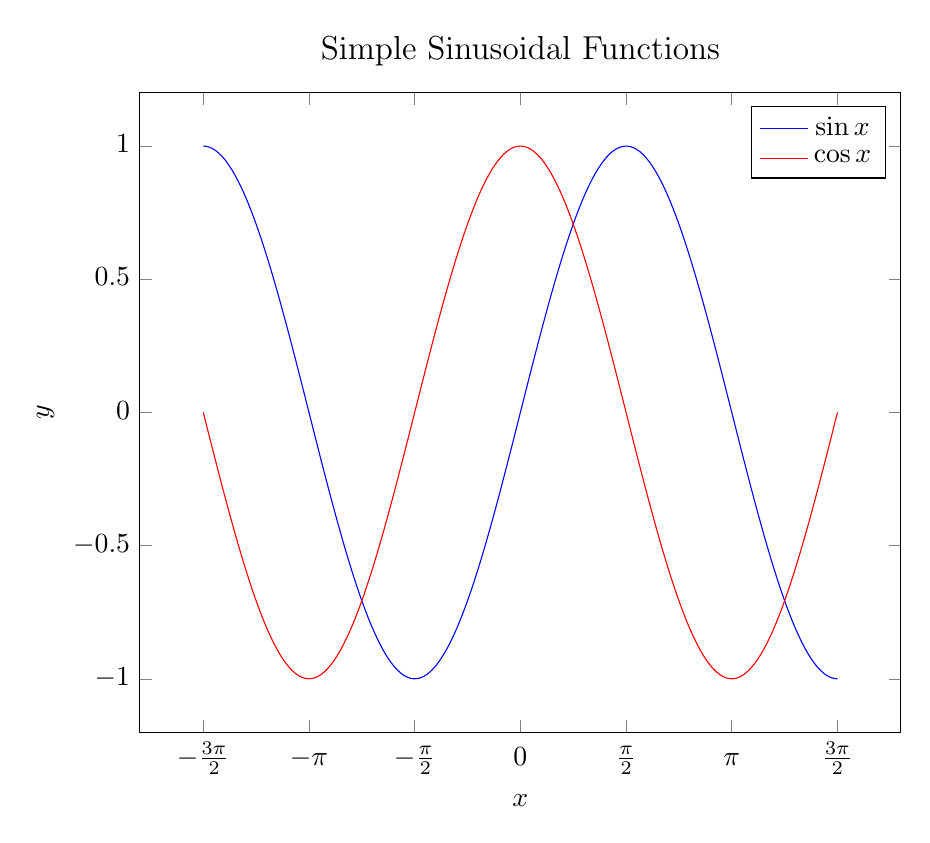
\begin{tikzpicture}
			\begin{axis}[
				height = 0.8*\textwidth,
				title = \large{Simple Sinusoidal Functions},
				xlabel = $x$,
				ylabel = $y$,
				xtick = {-1.5*pi, -pi, -pi/2, 0, pi/2, pi, 3*pi/2},
				xticklabels = {$-\frac{3\pi}{2}$, $-\pi$, $-\frac{\pi}{2}$, $0$, $\frac{\pi}{2}$, $\pi$, $\frac{3\pi}{2}$},
				typeset ticklabels with strut,
				xlabel near ticks]
				\addplot[domain = -1.5*pi:1.5*pi, samples=200, color=blue]{sin(180*x/pi)};
				\addlegendentry{$\sin x$}
				\addplot[domain = -1.5*pi:1.5*pi, samples=200, color=red]{cos(180*x/pi)};
				\addlegendentry{$\cos x$}
			\end{axis}
		\end{tikzpicture}
		\caption{Vector graphic made in \LaTeX}
		\label{fig:ExampleVectorImage}
	\end{subfigure}
	\caption{A comparison between a image rasterised with low-quality and a vector graphic.}
	\label{fig:ExamplePlots}
\end{figure}

Below is a list of other features of \LaTeX\ that make it better for writing technical documents that Word does not support.

\begin{itemize}
	\item Subfigures can be given automatically numbered with easily cross-referencable subcaptions.
	\item Figures and tables can be given an optional short caption which appears in the list of tables and list of figures. This means brief metadata about figures can be kept closely attached to the figures and tables in the caption without cluttering the corresponding lists.
	\item The exact positioning of objects is handled automatically. For example, the user provides the caption text and the compiler puts it in a sensible place.
	\item All formatting changes can be tracked and easily copied.
	\item Smaller file sizes and the ability to handle documents several hundred pages long easily.
	\item The output is determined exactly from the text input so it is not possible to reload the output and get different behaviour like in Word.
\end{itemize}\newpage
\section{Version Control}
\label{sec:VersionControl}

% Track changes in Word can cause many revisions, for example if remove space after paragraph is applied to a table then every cell will be a revision.
% Comparing git diff with current Word-based methods.
% Security and how you can self-host a git server.
% Log of changes - who made what change and when.
% Blobs are hashed. Can use signed commits to confirm what time commits were made.
% https://github.com/HenryGinn/Essays/tree/main/TheCaseForLaTeX

In this section I want to compare currently used version control methods for Word documents with what is possible with \LaTeX. One of the main powers of \LaTeX\ is that it is fully compatible with text-based version control software such as Git, the free and open source software used by almost all developers and software companies. Here we will not look at all the features of Git or how it works, but trust that it is more than powerful enough for the needs of WSP.

\subsection{Current Practice}

There are two main types of differences that someone may care about:

\begin{itemize}
	\item Changes in meaning such as ``Updated system description to comply with requirement xyz".
	\item All changes to the text and formatting.
\end{itemize}

On my current project we track the former in a table of changes and the latter with cross-through formatting and green highlighting. It may be the case that this project has a uniquely horrifying version control policy, but nonetheless it is worth highlighing the problems with it.

\begin{itemize}
	\item \textbf{Manually recording changes.} If someone forgets to record the change or incorrectly applies the formatting then the change is not properly tracked. As Git does this automatically it saves the need for the author to do it and also ensures it is always done correctly.
	\item \textbf{The document is harder to read.} The current version should not be polluted by the remnants of superseded parts. I regularly see paragraphs weaving in and out of superseded and non-superseded text which makes the current version hard to parse. It is not possible to easily see the document without the version control formatting either.
	\item \textbf{Updating revisions.} When a new revision is being prepared, the first task is to remove all text with cross-through formatting and remove all green highlight. This is a manual task that should not exist. As before, this process is also error prone - consider figure~\ref{fig:4Strikethrough} where it is almost impossible to see the difference between a four that has been removed from the document and one that has been added. Figure~\ref{fig:UnclearStrikethrough} has a single row that has been removed that could easily be missed when preparing the next revision.
	\item \textbf{Formatting.} Formatting in Word is often inherent to the subject of the formatting or is given by invisible characters\footnote{For example, the formatting of a bullet point or paragraph number is given by an invisible formatting character at the end of the clause and I have seen multiple people confused as to why they cannot clear highlighting from a previous revision.} so cannot be tracked by this method. Other changes in formatting such as the structure of a table can only be recorded by duplicating the whole table and applying cross-through formatting.
	\item \textbf{Confusion between types of change.} There is no distinction between the two types of changes making for useless tables of changes. I have seen sections completely rewritten with the description ``Text revised" and the tense of a single unimportant word changed where the letters that were added and removed were stated. Both of these examples followed the version control policy exactly.
\end{itemize}

\begin{figure}[!htb]
	% Store largest image in a box
	\savebox{\imagebox}{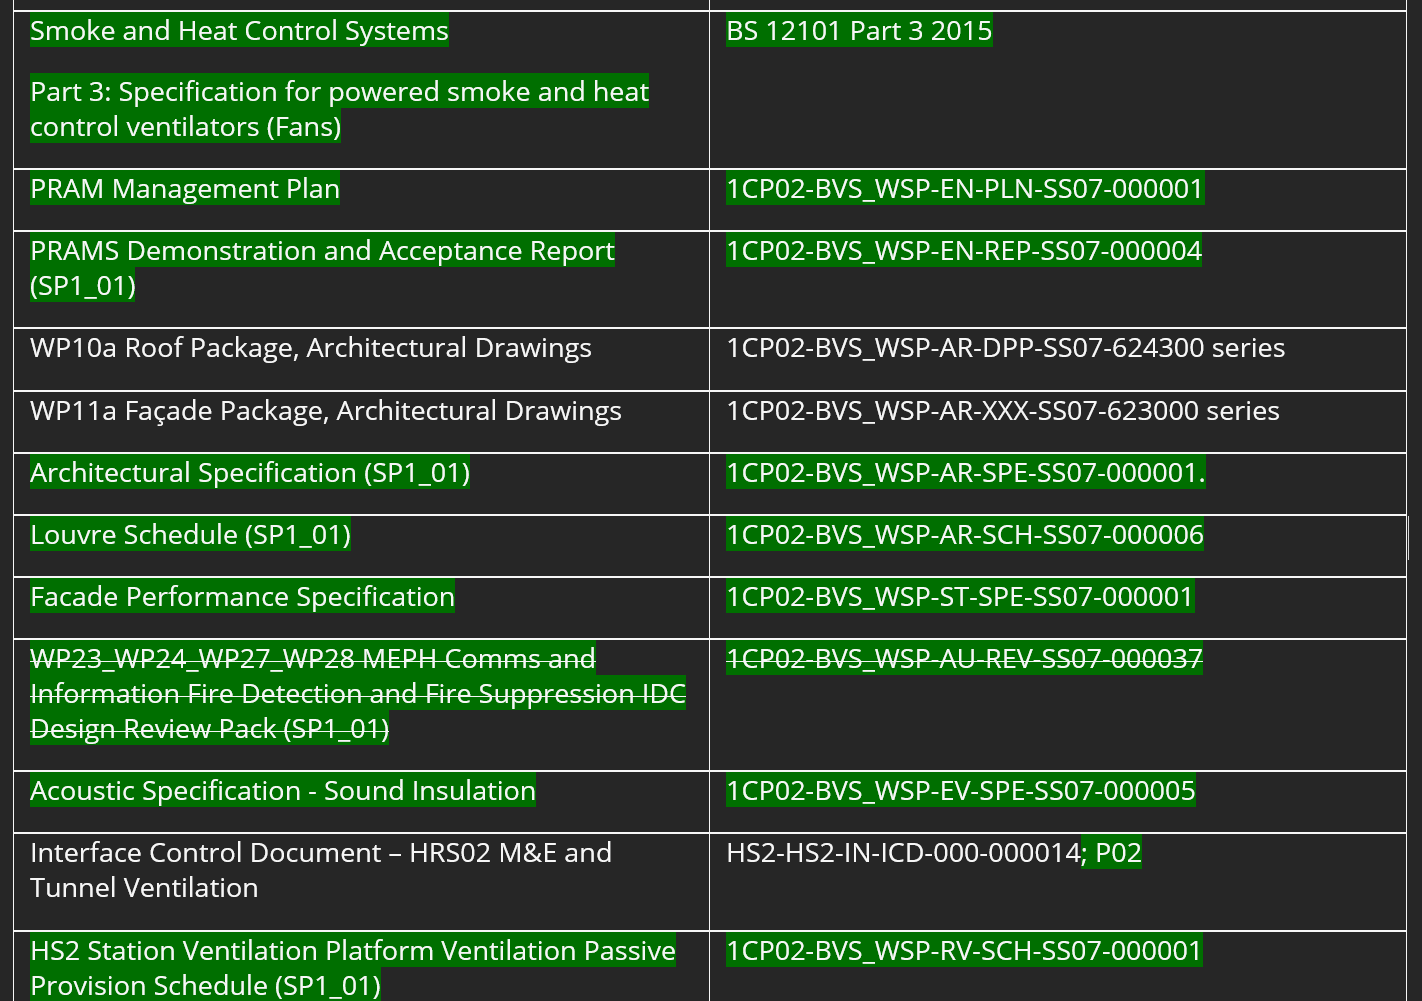
\includegraphics[width=0.75\textwidth]{Figures/ExampleOfPoorVersionControl.png}}
	\begin{subfigure}[t]{0.2\textwidth}
		\centering\raisebox{\dimexpr0.5\ht\imagebox-0.5\height}{% Raise smaller image into place
			
\includegraphics[width=\textwidth]{Figures/StrikethroughFour.png}}
			\caption{Strike-through comparison}
			\label{fig:4Strikethrough}
	\end{subfigure}
	\hfill
	\begin{subfigure}[t]{0.75\textwidth}
		\centering\usebox{\imagebox}% Place largest image
		\caption{Current version control example}
		\label{fig:UnclearStrikethrough}
	\end{subfigure}
	\caption{Examples of a current method of version control for Word documents.}
	\label{fig:WordVersionControl}
\end{figure}


\subsection{Resolution with \LaTeX\ and Git}

Let us see how an approach with \LaTeX\ and git avoids these problems. Before we look into how Git can avoid these issues we must first have some understanding of Git.

In short, after some changes are made the author creates something called a ``commit" which is a snapshot of the project at that point in time\footnote{Git does not store only the changes and it also does not create a copy of the whole project. It works in a clever way that is beyond the scope of this essay that means the total amount of stored data is small.}, and then this commit can be sent to a shared repository. \href{https://www.youtube.com/watch?v=e9lnsKot_SQ}{\underline{This video}} gives a simple explanation of the Git workflow for those wanting to know more.

The difference between any two commits can be produced on command is seen in figure~\ref{fig:ExampleOfDiff}.

\begin{figure}[!htb]
	\centering
	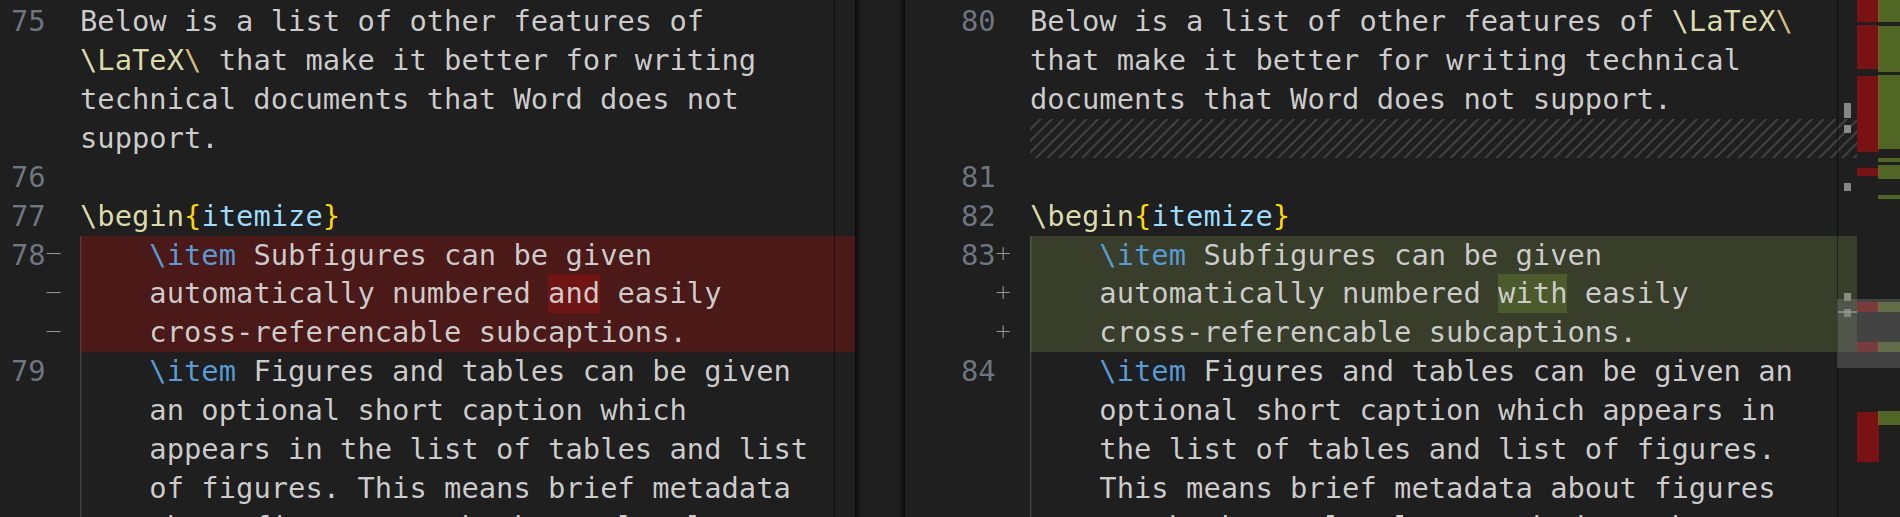
\includegraphics[width=\textwidth]{Figures/ExampleOfDiff2.png}
	\caption{An example of the difference between two files.}
	\label{fig:ExampleOfDiff}
\end{figure}

\LaTeX\ is also better for version control. As it is all text-based it can be used with version control software like Git, which gives tracability, control over branches, and easy computation of differences between versions. This also tracks any formatting changes that cannot be handled by the template such as the shape of a table.\newpage
\input{EaseOfUse.tex}\newpage
\section{Failures of Word}
\label{sec:FailuresOfWord}

In this section I want to give some examples of times where the use of Word has caused me significant grief which would never have been a problem when using a combination of \LaTeX\ and Git. Here I want to highlight how much time and energy is wasted by using Word. The section is concluded by a list of annoying behaviours of Word.

\subsection{Attaching PDF Documents in Appendices}
\label{subsec:AttachingPdfDocumentsInAppendices}

Several times I have had to attach spreadsheets as an appendix to a PDF as part of a deliverable\footnote{Personally I believe this is not best practice and we should be sending the native file, but we will ignore that.}. Below is the process we use to get the correct page numbers in the footer and table of contents and links that go to the intended page:

\begin{enumerate}
	\item Go to the first sheet of the spreadsheet being included, change the ``start at page number" setting to match the position it belongs in the document, and export it.
	\item Repeat this for the next sheets of the spreadsheet, ensuring that the page number adds the length of the previous sheets that have been converted to PDF.
	\item After the corresponding appendix title page, add blank pages equal to the length of the PDF being included.
	\item Repeat for all spreadsheets being included (or just step 3 for existing PDFs).
	\item After exporting Word to PDF, remove the blank pages in a pdf editor and add in the pages of the PDFs to be included.
\end{enumerate}

There are several problems with this approach. Firstly, this is an error-prone process. The chances of pages being added in the wrong order is high and there are many opportunities to end up with incorrect page numbers and table of contents links anyway. Secondly, if any changes to the document are made that change the length of the document then the whole process will need to be redone. Finally, this process can take a long time. I once complained to a colleague how I had ended up wasting a whole day converting a document to a PDF and they told me they had done the same thing before.

Let us consider how this works in \LaTeX. All sheets are exported to PDF without page numbers and there is a simple single line of code that tells the compiler to include a PDF with page numbers. All links and page numbers are done for you and are updated automatically in response to any changes. In addition to this, these page numbers (and any other header or footer information) will follow the document template given and would not need to be recreated in Excel.

\subsection{Version Control}
\label{subsec:VersionControl}

Recently I had a Sharepoint synced folder that stopped syncing and I did not notice for a month. This meant that several documents I was working on had diverged from the main version and I would need to merge any changes I had made into the main document. To be fully confident I had not missed anything, I needed to copy both documents into Notepad, remove the clause numbers to stop superfluous differences being detected, and then use a tool that identified differences between two texts. After this I had to check all formatting was correct because this method would not have been picked up formatting differences.

I ended up wasting a whole day on this task. As described in section~\ref{sec:VersionControl}, this was something that Git was designed for and would therefore have taken only a few minutes per document.

\subsection{Changing Template}

Recently a colleague had used a WSP template for some work where it was subsequently decided that it belonged in a document for the project, meaning changing to the project template. No matter what type of paste special I used, the styles of the project template would not apply and I needed to go through and apply the styles by hand. This was not too arduous for a 12-page document, but there were many tables that needed formatting. This should have been a case of applying the table header style to the header and the table body style to the body, but that did not work. Instead the font size, font type, font colour, font alignment, cell borders, cell alignment, and paragraph alignment had to be set manually, for both the header and the body for every table\footnote{This template uses a different font style and size for the header than the rest of the document. This would be awkward to do in \LaTeX\ because it is terrible typesetting practice.}.

I spent an afternoon fixing this. Using \LaTeX\ this would have been solved by a single copy and paste because the formatting is handled elsewhere. Worse, it turned out that my colleague had a more up-to-date version of the document stored locally, so I had to carefully scan for differences between the tables and update them manually. If using \LaTeX\ then I could have copy and pasted again.

\subsection{Assorted Complaints of Word}

In case it is not clear how unstable, buggy, and annoying Word is, I have included a few oddities and frustrations of Word below:

\begin{itemize}
	\item Tables split across page breaks by default.
	\item Captions are not attached to the corresponding object by default.
	\item Sometimes invisible, unselectable, and undeletable formatting characters can appear in your document that break your formatting. The only fix for this is awkwardly manoeuvering the character somewhere it does no harm or copying everything into a new document.
	\item Clicking the bullet point button can change the font size and font style.
	\item Space after paragraph should be used to ensure space between paragraphs, but the space is still added for the last paragraph on the page. As the space is attached to the paragraph, it puts the line on the next page even if that line would fit above. To avoid widows, space after paragraph needs to be manually handled.
	\item The gap between ``Figure" or ``Table" and the number in the caption is not a non-breaking space by default. This can result in the number being on a new line when cross-referencing.
	\item Vertically centred text in a cell of a table does not appear vertically centred, even if space before and after paragraph are the same and margins are symmetrical.
	\item Page breaks take up space. This means if the last line that fits on the page is long then the page break mark is moved to the next page, meaning a blank page. This means needing to manually handle the page break. This often occurs with tables and figures.
	\item Changing the width of a column in a table where the last cell highlighted is merged will only change the width of the first row of the merged cell. This means needing to change the width of those cells separately and remerging afterwards.
	\item The number of words that fit on a line depends on their justification - this should only affect the spacing between words (unless rivers are automatically avoided which Word cannot do).
	\item The default behaviour of images is ``keep with next", yet if two images will not fit on the same page together then word will put them on separate pages with an automatic page break on the preceeding page, even if there was room for the first image\footnote{If two images are meant to be understood together then they should be subfigures of a single figure object.}.
\end{itemize}\newpage
\section{Conclusion}
\label{sec:Conclusion}

In summary, it is far faster and easier to produce technical documents in \LaTeX\ once familiarity has been attained, and the results are of higher quality and appear more professional. Table~\ref{tab:Comparison} below gives a comparison of the key differences between Word and \LaTeX. The source code for this essay is available on my \href{https://github.com/HenryGinn/Essays/tree/main/TheCaseForLaTeX}{\underline{GitHub}}.

\begin{table}[H]
	\centering
	\caption{Comparing Word and \LaTeX.}
	\label{tab:Comparison}
	\begin{tabular}{ccc}
		\myhline
		Property & Word & \LaTeX  \\
		\myhline
		Editor format & What You See Is What You Get & Needs to compile  \\
		Bugfixing & Poor support and confusing behaviour & Good support with searchable errors  \\
		Software & Proprietary & Free and Open Source  \\
		Formatting control & Poor & High  \\
		Technical features & Lacking & Rich  \\
		Microsoft compatibility & High & Medium  \\
		Simplicity & Extremely simple &  $\sim$~1 hour of training  \\
		Version control & Medium & Git-compatible  \\
		\myhline
	\end{tabular}
\end{table}

\LaTeX\ is standard software in academia. Git is standard software in software engineering. They are both extremely mature and have been successfully implemented in these sectors so I see no reason why this could not also be the case in engineering and consultancy. Collaboration, version control, and producing technical documents is a hard problem, but it has been solved by \LaTeX\ and Git. Therefore I hope that WSP agrees that their use is inline with their digitial approach and considers implementing this technology.

\end{document}